\section{函数的极限}
\label{sec:analysis-function-limits}

数列的指标按自然数逐项增加，函数的输入却可以从许多实数位置靠近同一点。例如$(x^2-1)/(x-1)$在$x=1$没有定义，但在$x\neq1$时它等于$x+1$，所以邻近输入的输出仍趋于$2$。函数极限研究的正是这种去掉中心点后的共同趋近，不要求函数在中心有取值。

\subsection{函数极限的定义}
\paragraph{聚点}

讨论输入接近$a$之前，须保证定义域中确实有不同于$a$的输入能够任意靠近$a$。
设$X\subseteq\mathbb R$。若每个$r>0$都能找到$x\in X$使$0<|x-a|<r$，
即$(a-r,a+r)$去掉$a$以后（称为$a$的去心邻域）总含有$X$中的点，就称$a$为$X$的\term{聚点}（cluster point）。
例如$0$是$(0,1)$的聚点，虽然$0$不属于这个集合。
$X$中不是聚点的点称为$X$的\term{孤立点}（isolated point），例如整数集合中的每个点；
在孤立点附近没有其他输入，谈不上“趋近”。

\paragraph{函数极限}
有了能够趋近的输入，还要用输入误差控制输出误差，这与数列极限比较尾部误差的思路相同。
设$f:X\to\mathbb R$，$a$为$X$的聚点，$b\in\mathbb R$。
若对每个$\varepsilon>0$，都存在$\delta>0$使
\[
 x\in X,\quad0<|x-a|<\delta\quad\Longrightarrow\quad|f(x)-b|<\varepsilon,
\]
就称$b$为$x\to a$时$f(x)$的极限，记作$\lim_{x\to a}f(x)=b$。
也就是说，只要输入与$a$足够近，输出与$b$的距离就能任意小。

定义中的$0<|x-a|$排除了中心点，所以既不要求$f(a)$有定义，也不要求它等于$b$。
回到开头的例子$f(x)=(x^2-1)/(x-1)$：对$x\neq1$有$f(x)=x+1$。
给定$\varepsilon>0$，取$\delta=\varepsilon$，则
$0<|x-1|<\delta$时$|f(x)-2|=|x-1|<\varepsilon$，所以其极限为$2$。

图~\ref{fig:analysis-process-epsilon-delta-band}将输入邻域与输出误差带对应起来，同时把基点取值与趋近时的极限分开。
\begin{figure}[!htbp]
 \centering
 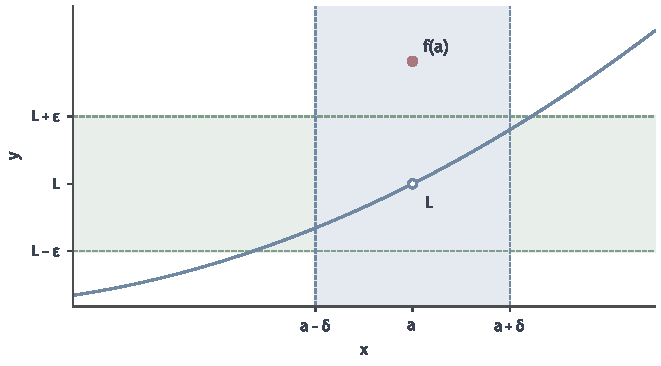
\includegraphics[width=112.0mm]{figures/00-shared/mathematical-preliminaries-upper/00-shared/matplotlib/chapter3-concept-processes/epsilon-delta-band.pdf}
 \caption{取$a=L=1$（$L$即正文中的极限值$b$），$x\neq1$时$f(x)=x^2$，另令$f(1)=2$。蓝带对应$\delta=0.2$的输入范围，绿带对应$\varepsilon=0.55$的输出范围；去掉$a$后，蓝带内曲线全部落在绿带内。空心点是极限位置，红实心点是$f(a)$，不参加去心邻域条件。}
 \label{fig:analysis-process-epsilon-delta-band}
\end{figure}

\paragraph{左极限与右极限}
实轴上的输入可以从一个点的两侧接近，而两侧的输出未必有相同趋向，因此先分别考察每一侧的极限。
只让$x<a$的点趋近$a$，得到左极限$\lim_{x\uparrow a}f(x)$；
只让$x>a$的点趋近$a$，得到右极限$\lim_{x\downarrow a}f(x)$。
两种定义分别在上述误差条件中增加$x<a$或$x>a$，
并要求相应一侧存在定义域中的点任意靠近$a$。
若两侧都能趋近$a$，双侧极限存在当且仅当左右极限都存在且相等。

例如$f(x)=\mathbb I\{x\geq0\}$在$0$处的左右极限分别为$0$和$1$，所以双侧极限不存在。
这里$\mathbb I$为指示函数：括号内条件成立时取$1$，否则取$0$。
在定义域$[a,b]$内，只能从右侧趋近左端点$a$，从左侧趋近右端点$b$。
这种左右判据依赖实轴上的顺序，多元函数还须控制其他趋近方式。

\paragraph{无穷远处的极限}
输入也可以趋于无穷。设定义域向右无界，条件
\[
 \lim_{x\to+\infty}f(x)=b
\]
表示：对每个$\varepsilon>0$，存在$M$，使定义域中所有$x>M$都满足$|f(x)-b|<\varepsilon$。
定义域向左无界时，$x\to-\infty$的定义相应要求所有$x<M$的允许输入满足同一误差界。
例如$1/x$在$x\to+\infty$和$x\to-\infty$时都趋于$0$。

\paragraph{值为无穷的极限}
前一段改变的是输入的趋向；即使输入趋近有限点，输出也可能越过任何有限界，因此还需要描述输出本身的无界趋向。
对有限聚点$a$，$f(x)\to+\infty$（$x\to a$）是指：对每个实数$M$，都存在$\delta>0$，使定义域中满足$0<|x-a|<\delta$的每个$x$都有$f(x)>M$。
趋于$-\infty$则把最后的不等式改为$f(x)<M$。单侧无穷极限再限制输入所在的一侧。
因此$1/x$在$x\downarrow0$时趋于$+\infty$，在$x\uparrow0$时趋于$-\infty$，并没有共同的双侧无穷极限。

\subsection{常见函数的极限}

\paragraph{三角函数}
三角函数的自变量采用弧度制：单位圆上弧长为$h$的圆心角记为$h$。
比较内接三角形、扇形和外切三角形的面积，可得$0<h<\pi/2$时
$\sin h\leq h\leq\tan h$，从而$\cos h\leq\sin h/h\leq1$。
又由$1-\cos h=2\sin^2(h/2)\leq h^2/2$得到误差界
\[
 0\leq1-\frac{\sin h}{h}\leq1-\cos h\leq\frac{h^2}{2}.
\]

任给$\varepsilon>0$，只要$0<h<\min\{\pi/2,\sqrt{2\varepsilon}\}$，第一个比值与$1$的误差就小于$\varepsilon$；
$\sin h/h$是偶函数，所以同一估计也控制$h<0$的一侧。
第二个比值由$|1-\cos h|/|h|\leq|h|/2$控制，这个误差界对正负两侧都适用。因此
\[
 \lim_{h\to0}\frac{\sin h}{h}=1,
 \qquad
 \lim_{h\to0}\frac{\cos h-1}{h}=0.
\]
弧度制使第一个极限恰为$1$，用角度制时会多出比例系数。

\paragraph{自然指数函数}
后面求指数函数的导数需要一个原点处的基本极限。下面先用级数构造自然指数函数并验证其收敛，
再建立乘法性质和局部变化关系。定义
\[
 \exp x=\sum_{k=0}^{\infty}\frac{x^k}{k!}.
\]
对固定$x$，相邻项绝对值之比为$|x|/(k+1)$，当$k+1\geq2|x|$时不超过$1/2$，
尾部被几何级数控制，所以级数绝对收敛。

为得到乘法性质，先考察两个绝对收敛级数$\sum_k a_k$与$\sum_j b_j$的乘积。有限的正方形和满足
$\sum_{k=0}^N\sum_{j=0}^Na_kb_j=(\sum_{k=0}^Na_k)(\sum_{j=0}^Nb_j)$，
所以它们趋于两级数和的乘积。按总次数$k+j=n$合并的三角形部分和$\sum_{n=0}^{N}\sum_{k+j=n}a_kb_j$，
与正方形和只差满足$k,j\leq N$、$k+j>N$的项；这些项的$k$或$j$大于$N/2$，其绝对值之和不超过
$(\sum_{k>N/2}|a_k|)(\sum_j|b_j|)+(\sum_k|a_k|)(\sum_{j>N/2}|b_j|)$，它随$N$增大趋于零。
因此按总次数合并后也得到同一极限。

把这个结论用于指数级数，记
$C_n=\sum_{k=0}^n x^ky^{n-k}/[k!(n-k)!]$。将系数$n$拆为$k+(n-k)$，并分别换一次有限求和的索引，得到
\[
 nC_n=(x+y)C_{n-1},\qquad n\geq1.
\]
由$C_0=1$逐步得到$C_n=(x+y)^n/n!$，因而
\[
 \exp x\,\exp y
 =\sum_{n=0}^{\infty}\sum_{k=0}^n\frac{x^ky^{n-k}}{k!(n-k)!}
 =\sum_{n=0}^{\infty}\frac{(x+y)^n}{n!}
 =\exp(x+y).
\]
记$e=\exp1$，$e$约为$2.71828$。由加法公式，对正整数$n$有$\exp n=e^n$，
因此通常把$\exp x$写作$e^x$，称为以$e$为底的指数函数。

当$0<|h|<1/2$时，利用$1/k!\leq1$直接估计级数的二阶以后各项：
\[
 |e^h-1-h|
 \leq\sum_{k=2}^{\infty}|h|^k
 =\frac{h^2}{1-|h|}\leq2h^2.
\]
除以$|h|$得$|(e^h-1)/h-1|\leq2|h|$，令$h\to0$，就有
\[
 \lim_{h\to0}\frac{e^h-1}{h}=1.
\]
这一推导只用到级数，未使用求导或积分。

加法公式还给出其他性质。由$e^xe^{-x}=e^0=1$知$e^x\neq0$，又$e^x=(e^{x/2})^2\geq0$，因此$e^x>0$。
对$u\geq0$，级数各项非负，只保留前两项便得
\[
 e^u\geq1+u\qquad(u\geq0),
\]
这一不等式给出指数函数在非负半轴上的一个线性下界。
对$h>0$，由此$e^h\geq1+h>1$，于是$e^{x+h}=e^xe^h>e^x$，指数函数严格递增。
同一估计说明$x\to+\infty$时$e^x\to+\infty$；由$e^x=1/e^{-x}$又得$x\to-\infty$时$e^x\to0$。
对固定$x$和$|h|<1/2$，上述余项界还给出$|e^{x+h}-e^x|=e^x|e^h-1|\leq e^x(|h|+2h^2)\to0$。
这些性质将在连续函数的介值定理建立后，用于构造自然对数这一反函数
\scite{math-lebl-analysis1}。

\subsection{函数极限的性质与运算}
\paragraph{序列判据}

函数极限要求控制$a$附近所有允许的输入。这个条件等价于：每列满足$x_n\in X\setminus\{a\}$且$x_n\to a$的输入，都有$f(x_n)\to b$。

正向，给定$\varepsilon$后取函数极限中的$\delta$，充分靠后的$x_n$满足$0<|x_n-a|<\delta$，于是$|f(x_n)-b|<\varepsilon$。
反向用反证法。若误差条件不成立，就存在$\varepsilon_0>0$，使每个$1/n$去心邻域内都能选到$x_n\in X$，满足$|f(x_n)-b|\geq\varepsilon_0$；
这列输入趋于$a$，输出却不趋于$b$，与序列条件矛盾。

\paragraph{和的极限}
序列判据把函数极限转化为数列极限，从而可以逐项借用数列极限的运算法则。
以下各段统一设$f,g:D\to\mathbb R$，$a$为$D$的聚点，且在$x\in D$、$x\to a$时
$f(x)\to b$、$g(x)\to c$，其中$b,c\in\mathbb R$。和的极限为
\[
 \lim_{x\to a}(f(x)+g(x))=b+c.
\]
任取$x_n\in D\setminus\{a\}$且$x_n\to a$，序列判据给出$f(x_n)\to b$、$g(x_n)\to c$；
数列和的法则给出$f(x_n)+g(x_n)\to b+c$。由于对任意这样的输入列都成立，再用序列判据即得结论。

\paragraph{差的极限}
相减也保留有限极限关系：
\[
 \lim_{x\to a}(f(x)-g(x))=b-c.
\]
对每列趋于$a$的允许输入，数列差的法则都给出相应输出差趋于$b-c$，再由序列判据返回函数极限。

\paragraph{数乘的极限}
固定倍数只按比例改变输出误差。对任意固定$\lambda\in\mathbb R$，
\[
 \lim_{x\to a}\lambda f(x)=\lambda b.
\]
沿任意允许输入列使用数列常数倍的极限，再用序列判据即可；$\lambda=0$时输出恒为零。

\paragraph{积的极限}
两个有限极限也可以分别相乘：
\[
 \lim_{x\to a}f(x)g(x)=bc.
\]
沿任意允许输入列应用数列乘积的法则，得到输出积趋于$bc$；序列判据保证这控制了$a$附近的全部允许输入。

\paragraph{商的极限}
商需要额外要求分母极限$c\neq0$，此时
\[
 \lim_{x\to a}\frac{f(x)}{g(x)}=\frac bc.
\]
先取输出误差$|c|/2$，便知$a$的某个去心邻域内有$|g(x)|>|c|/2>0$，商在那里有定义。
在这一邻域内，任意输入列都可使用数列的商法则，再由序列判据得到结论。

若分子分母都趋于零，就不能套用此式。例如$(x^2-1)/(x-1)$在$x\to1$时须先约去公因子$x-1$，才能求出极限$2$。
同样，$\infty-\infty$等形式也须先变形或另外估计。

\paragraph{夹逼定理}
不易直接分解的函数，可以用同趋向的两侧函数控制。设在$a$的某个去心邻域内，所有允许输入满足
$u(x)\leq h(x)\leq v(x)$，且$u(x)\to L$、$v(x)\to L$，其中$L\in\mathbb R$，则
\[
 \lim_{x\to a}h(x)=L.
\]
任给$\varepsilon>0$，取一个共同的去心邻域，使其中$u(x)$和$v(x)$都落在$(L-\varepsilon,L+\varepsilon)$内，
夹在中间的$h(x)$也在其中。例如$-|x|\leq x\sin(1/x)\leq|x|$在$x\neq0$时成立，因此$x\to0$时$x\sin(1/x)\to0$。

\subsection{无穷小与无穷大}

\paragraph{无穷小}
趋向零的量可以出现在数列、函数或后面的微分余项中，先给这类趋向一个统一名称。
在指定的趋向下，极限为$0$的函数（或数列）称为无穷小（infinitesimal）。
例如$x\to0$时，$x$和$x^2$都是无穷小；$n\to\infty$时，$1/n$也是无穷小。
“无穷小”描述变化过程中的极限性质，不是某个固定的很小的非零数。

\paragraph{无穷大}
函数值的绝对值也可能最终超过任意固定门槛，这种趋向与趋零可以通过倒数联系起来。
在指定的趋向下，若$|f(x)|\to+\infty$，则称$f$为无穷大。
例如$x\to0$时，$1/x$为无穷大，但它没有共同的正或负无穷极限。
若$f$在所考察的趋向附近非零，则$|f|\to+\infty$等价于$1/f\to0$。

\paragraph{渐近记号}
\label{sec:comb-growth-scales}
两个函数即使同为无穷小，趋零的相对速度也可以不同。
设在所讨论的趋向附近$g\neq0$，定义
\[
 f=o(g)\quad\text{表示}\quad \frac{f}{g}\longrightarrow0.
\]
这个小$o$记号表示$f$相对于$g$可以忽略。
若$|f/g|$在趋向附近有界，则记$f=O(g)$，称为大$O$记号。
大$O$只要求有常数$C$使$|f|\leq C|g|$最终成立，小$o$则要求这个相对比例趋于零。
例如$x\to0$时$x^2=o(x)$，而$3x=O(x)$但不是$o(x)$。
若$f/g\to1$，还记$f\sim g$；两者都趋零时，称为等价无穷小。
例如$x\to0$时$x+x^2\sim x$，因为$(x+x^2)/x=1+x\to1$。

同样的记号可用于$n\to\infty$的数列：
$3n+7=O(n)$、$n/10=O(n)$，但这两个比值分别趋于$3$和$0.1$，所以都不是$o(n)$；
$10\sqrt n=o(n)$，因为$10\sqrt n/n=10/\sqrt n\to0$。
图~\ref{fig:vol1-add-asymptotic-ratios}画出这三个比值。

\begin{figure}[!htb]
  \centering
  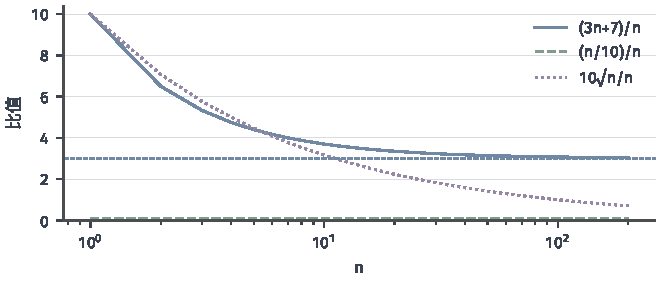
\includegraphics[width=112mm]{figures/00-shared/mathematical-preliminaries-upper/00-shared/matplotlib/mathematical-language-combinatorics-analysis-optimization-comprehension-additions/asymptotic-ratios.pdf}
  \caption{三个解析数列除以$n$后的比值，展示整数$n=1,\ldots,200$，横轴为对数刻度。蓝、绿、紫线的极限分别为$3,0.1,0$。前两者对应$O(n)$而非$o(n)$，第三者对应$o(n)$；极限由正文中的表达式判断，有限范围曲线只帮助观察。}
  \label{fig:vol1-add-asymptotic-ratios}
\end{figure}

对最终为正的数列，若存在$c>0$使$a_n\geq cb_n$最终成立，记$a_n=\Omega(b_n)$；
同时满足$a_n=O(b_n)$与$a_n=\Omega(b_n)$，记$a_n=\Theta(b_n)$，表示同一数量级。
例如$3n+7=\Theta(n)$。这里的常数不随趋于无穷的$n$改变。
$n=O(n^2)$也成立，因此大$O$给出上界，不一定给出精确的增长阶。
这些记号在求导和局部近似中用来表达余项的大小。

\FloatBarrier
